\documentclass[9pt,a4paper]{extarticle}


	\usepackage[margin=5em,bottom=8em]{geometry}


%1 est la marge gauche
%2 est la marge en haut
%3 est la marge droite
%4 est la marge en bas
%5 fixe la hauteur de l'entête
%6 fixe la distance entre l'entête et le texte
%7 fixe la hauteur du pied de page
%8 fixe la distance entre le texte et le pied de page
%------------------------------Packages généraux------------------------------

\usepackage[english]{babel}
\usepackage[T1]{fontenc}
\usepackage{ae}
\usepackage[utf8]{inputenc}
\usepackage{scrextend}
\usepackage{hyperref}
 \hypersetup{
    colorlinks = true,
    linkcolor=black,
    urlcolor = black
    }
%-------------------------Mathématiques------------------------------
\usepackage{amsmath}
\usepackage{amssymb}
\usepackage{amsthm}
\usepackage{amsfonts}
\usepackage{eucal}
\newcommand\independent{\protect\mathpalette{\protect\independenT}{\perp}}
\def\independenT#1#2{\mathrel{\rlap{$#1#2$}\mkern2mu{#1#2}}}
%-----------------------Codes et algorithmes--------------------------
\usepackage{algorithm}
%\usepackage{algorithmic}
%\usepackage{clrscode3e}
\usepackage[noend]{algpseudocode}
%\newcommand{\pushline}{\Indp}% Indent
%\newcommand{\popline}{\Indm\dosemic}% Undent
%\newcommand{\nonl}{\renewcommand{\nl}{\let\nl\oldnl}}%


%------------------------------Graphics------------------------------

\usepackage{graphicx}
\usepackage{fancyhdr}
\usepackage{fancybox}
\usepackage{color}
\usepackage{pgf, tikz}
\usetikzlibrary{arrows, automata}
%\usepackage{slashbox}

%------------------Sub-sections--------%
\usepackage{titlesec}
\usepackage{hyperref}
\usepackage{comment}

\usepackage{hyperref}
\usepackage{qrcode}
               
 \hypersetup{
    colorlinks = true,
    linkcolor=black,
    urlcolor = black
    }
    
\newenvironment{solution}
    {%\begin{center}
    %\begin{tabular}{|p{0.9\textwidth}|}
    %\hline\\
    \color{red}
    }
    { 
    %\\\\\hline
    %\end{tabular} 
    %\end{center}
    \color{black}
    }
    
\newcommand{\blue}[1]{\textcolor{blue}{#1}}


\newif\ifhideproofs
\hideproofstrue %uncomment to hide proofs

\ifhideproofs
\usepackage{environ}
\NewEnviron{hide}{}
\let\solution\hide
\let\endsolution\endhide
\fi

\title{{\bf INFO8006 Introduction to Artificial Intelligence}\\[1em]
Exercises 4: Reasoning under uncertainty (part 1)}
\date{}
%------------------------------Début du document------------------------------
\begin{document}
\maketitle
\vspace{-4em}
%------------------------------Page de garde------------------------------

  \section*{Learning outcomes}
      At the end of this exercice session you should be able to:
      \begin{itemize}
          \item Apply the Bayes rule and marginalisation appropriately to compute probabilities.
      \end{itemize}
   \section*{Exercise 1 (AIMA, Ex 13.4)}
   Let the two events $A, B$ of the probability space $\Omega$. Would it be rational for an agent to hold the three beliefs $P(A)=0.4$, $P(B)=0.3$, and
    $P(A\vee B)=0.5$? If so, what range of probabilities be rational for the agent to hold for $A\wedge B$?
    \begin{solution}
    % Definition of circles
\def\firstcircle{(0,0) circle (1.5cm)}
\def\secondcircle{(0:2cm) circle (1.5cm)}

\colorlet{circle edge}{blue!50}
\colorlet{circle area}{blue!20}

\tikzset{filled/.style={fill=circle area, draw=circle edge, thick},
    outline/.style={draw=circle edge, thick}}

\setlength{\parskip}{5mm}
% Set A and B
\begin{tikzpicture}
    \begin{scope}
        \clip \firstcircle;
        \fill[filled] \secondcircle;
    \end{scope}
    \draw[outline] \firstcircle node {$A$};
    \draw[outline] \secondcircle node {$B$};
    \node[anchor=south] at (current bounding box.north) {$A \cap B$};
\end{tikzpicture}

% Set A or B
\begin{tikzpicture}
    \draw[filled] \firstcircle node {$A$}
                  \secondcircle node {$B$};
    \node[anchor=south] at (current bounding box.north) {$A \cup B$};
\end{tikzpicture}

Yes it is possible, $P(A \land B) = P(A) + P(B) - P(A \lor B) = 0.4 + 0.3 - 0.5 = 0.2$
    \end{solution}
    \section*{Exercise 2 (AIMA, Ex 13.8)}
    Given the probability table of Table \ref{tab:p_table} compute the following probabilities:
    \begin{enumerate}
        \item P(toothache)
        \item P(cavity)
        \item P(toothache | cavity)
        \item P(cavity | toothache $\vee$ catch)
    \end{enumerate}
    \begin{solution}
    \begin{itemize}
        \item $P(T=t) = \sum_{i \in \{ct, \lnot ct\}}\sum_{j \in \{cv, \lnot cv\}}P(T=t, CT=i, CV=j) = 0.108 + 0.012 + 0.016 + 0.064 = 0.2$
        \item $P(CV=cv) = \sum_{i \in \{ct, \lnot ct\}}\sum_{j \in \{t, \lnot t\}}P(T=j, CT=i, CV=cv) = 0.108 + 0.012 + 0.072 + 0.008 = 0.2$
        \item $P(T=t|CV=cv) = \frac{P(T=t, CV=cv)}{P(CV=cv)} = \frac{\sum_{i \in \{ct, \lnot ct\}} P(T=t, CV=cv, CT=ct) }{P(CV=cv)} = \frac{0.108 + 0.012}{0.2} = 0.6$
        \item $P(T=t|CV=\lnot cv) = \frac{P(T=t, CV=\lnot cv)}{P(CV=\lnot cv)} = \frac{\sum_{i \in \{ct, \lnot ct\}} P(T=t, CV=\lnot cv, CT=ct) }{P(CV=cv)} = \frac{0.016 + 0.064}{0.8} = 0.1$
        \item $P(CV=cv|T=t \lor CT = ct) = \frac{P(CV=cv, T=t, CT=\lnot ct) + P(CV=cv, T=\lnot t, CT=ct) + P(CV=cv, T=t, CT=ct)}{\sum_{i \in \{cv, \lnot cv\}} P(CV=i, T=t, CT=\lnot ct) + P(CV=i, T=\lnot t, CT=ct) + P(CV=i, T=t, CT=ct)} = \frac{0.192}{0.192 + 0.224} = 0.46$
    \end{itemize}
    \end{solution}
    \begin{table}[H]
        \centering
        \begin{tabular}{|c|c|c|c|c|}
            \hline
             & \multicolumn{2}{c|}{Toothache} & \multicolumn{2}{c|}{$\lnot$ Toothache} \\ \hline
             & catch & $\lnot$ catch & catch & $\lnot$ catch \\ \hline
             cavity & $0.108$ & $0.012$ & $0.072$ & $0.008$ \\ \hline
             $\lnot$ cavity & $0.016$ & $0.064$ & $0.144$ & $0.576$ \\ \hline
        \end{tabular}
        \caption{Probablity Table of Toothache and Cavity.}
        \label{tab:p_table}
    \end{table}
\section*{Exercise 3:  Green Party President (\href{http://ai.berkeley.edu/sections/section_7_solutions_sp14.pdf}{Berkeley CS188 Spring 2014})}
It’s election season, and the chosen president may or may not be the Green Party candidate. Pundits (experts) believe that Green Party presidents are more likely to legalise marijuana than candidates from other parties, but legalisation
could occur under any administration. Armed with the power of probability, the analysts model the situation with the Bayes Net below.
\begin{figure}[h]
\centering

\begin{minipage}{.45\textwidth}
\centering
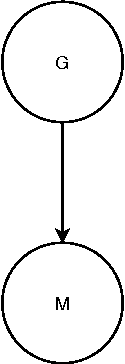
\includegraphics[width=.2\textwidth]{figures/GPP_bnet.pdf}
\end{minipage}
\begin{minipage}{.45\textwidth}
\centering
\begin{tabular}{c|c|c|}
         & $g$ & $\lnot g$ \\ \hline
         $P(G)$ & $.1$ & $.9$  
\end{tabular}

\begin{tabular}{c|c|c|}
         & $P(m|G)$ & $P(\lnot m|G)$ \\ \hline
         $g$ & $.667$ & $.333$ \\
         $\lnot g$ & $.25$ & $.75$ 
\end{tabular}
\end{minipage}
\end{figure}
\begin{enumerate}
    \item What is $P(M=m)$, the marginal probability that marijuana is legalised?
    \begin{solution}\\
    $P(M=m) = P(M=m, G=g) + P(M=m, G=\lnot g) = P(M=m| G=g)P(G=g) + P(M=m| G=\lnot g)P(G=\lnot g) = \frac{2}{3} \frac{1}{10} + \frac{1}{4} \frac{9}{10} = \frac{7}{24}$
    \end{solution}
    \item News agencies air 24/7 coverage of the recent legalisation of marijuana ($M=m$), but you can’t seem to find out who won the election. What is the conditional probability $P(G=g | M=m)$ that a Green Party president was elected?
    \begin{solution}\\
    $P(G=g|M=m) = \frac{P(G=g, M=m)}{P(M=m)} = \frac{P(M=m|G=g)P(G=g)}{P(M=m)} = \frac{\frac{2}{3}\frac{1}{10}}{\frac{7}{24}} = \frac{8}{35}$
    \end{solution}
    \item Fill in the joint probability table over G and M.
    \begin{solution}\\
    \begin{tabular}{|c|c|c|}
    \hline
         $G$ & $M$ & $P(G, M)$\\ \hline
         $g$ & $m$ & $\frac{1}{15}$\\ \hline
         $\lnot g$ & $m$ & $\frac{1}{30}$\\ \hline
         $g$ & $\lnot m$ & $\frac{9}{40}$\\ \hline
         $\lnot g$ & $\lnot m$ & $\frac{27}{40}$\\ \hline
         
    \end{tabular}
    \end{solution}
    
\end{enumerate}

\section*{Exercise 4 (AIMA, Ex 13.15)}
    After your yearly checkup, the doctor has bad news and good news. The bad news
is that you tested positive for a serious disease and that the test is 99\% accurate (i.e., the probability of testing positive when you do have the disease is 0.99, as is the probability of testing negative when you don’t have the disease). The good news is that this is a rare disease, striking only 1 in 10,000 people of your age. Why is it good news that the disease is rare? What are the chances that you actually have the disease?
\begin{solution}
It is a good news because the conditional probability will drop due to the weak prior value. We have $P(T=t | D=d) = P(T=\lnot t | D=\lnot d) = 0.99)$ and $P(D=d) = 10^{-4}$ and so:
$$ P(D=d|T=t) = \frac{P(T=t | D=d) P(D=d)}{P(T=t | D=d) P(D=d) = P(T=t | D= \lnot  d) P(D=\lnot d)} = \frac{0.99\times 10^{-4}}{0.99\times 10^{-4} + (1 - 0.99) \times (1 - 10^{-4})} = 0.0098$$
\end{solution}
\section*{Exercise 5 $\star$ (AIMA, Ex 13.3)}
For each of the following statements, either prove it is true or give a counterexample.
\begin{enumerate}
    \item If $P(a|b,c) = P(b|a, c),$ then $P(a|c) = P(b|c)$
    \item If $P(a|b,c) = P(a),$ then $P(b|c) = P(b)$
    \item If $P(a|b) = P(a),$ then $P(a|b, c) = P(a|c)$
\end{enumerate}
\begin{solution}
\begin{enumerate}
    \item True. By the product rule we know $P (b, c)P (a|b, c) = P (a, c)P (b|a, c)$, which by assumption reduces to $P (b, c) = P (a, c)$. Dividing through by $P (c)$ gives the result.
    \item False. The statement $P (a|b, c) = P (a)$ merely states that a is independent of b and c, it makes no claim regarding the dependence of b and c. A counter-example: $a$ and $b$ record the results of two independent coin flips, and $c = b$.
    \item False. While the statement $P (a|b) = P (a)$ implies that $a$ is independent of $b$, it does not imply that $a$ is conditionally independent of $b$ given $c$. A counter-example: $a$ and $b$ record the results of two independent coin flips, and $c$ equals the xor of $a$ and $b$.
\end{enumerate}
\end{solution}
\section*{Exercise 6 $\star$ (AIMA, Ex 13.6)}
Prove $ P(a\lor b) = P(a) + P(b) - P(a\land b) $ from Kolmogorov axioms.
\begin{solution}
\begin{align}
    P(a \lor b) &= p_{a,b} +p_{a,\lnot b} +p_{\lnot a,b} \\
    P(a) &= p_{a,b} + p_{a, \lnot b}\\
    P(b) &= p_{a,b}+p_{\lnot a,b}\\
    P(a\land b) &= p_{a,b} 
\end{align}
\end{solution}

   \section*{Supplementary materials}
   \begin{tabular}{c c}
       \href{https://www.youtube.com/watch?v=x-2uVNze56s}{Bayesian or Frequentist ?} & \qrcode{https://www.youtube.com/watch?v=x-2uVNze56s} \\
       AIMA 13.6 The wumpus world revisited & \\
       AIMA Chapter 13
   \end{tabular}

 
   
   
\end{document}
